This is part of the 2024 FDD of Team Tachyon e.V..
This is part of the FDD of Team Tachyon, file: coverpageEHW.tex
\newline
\newline

%An attempt to visualize a maglev train to show tikz.

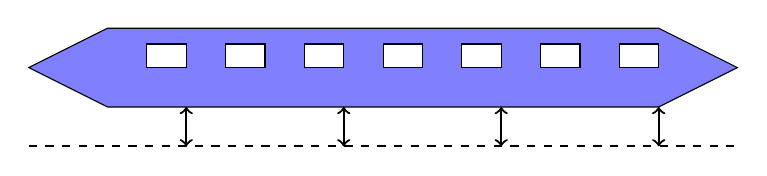
\begin{tikzpicture}
    % Train body
    \draw[fill=blue!50] (0,1) -- (1,1.5) -- (8,1.5) -- (9,1) -- (8,0.5) -- (1,0.5) -- cycle;
    % Levitation effect
    \draw[<->,thick] (2,0) -- (2,0.5);
    \draw[<->,thick] (4,0) -- (4,0.5);
    \draw[<->,thick] (6,0) -- (6,0.5);
    \draw[<->,thick] (8,0) -- (8,0.5);
    % Track
    \draw[thick,dashed] (0,0) -- (9,0);
    
    % Windows
    \foreach \x in {1.5,2.5,...,7.5} {
        \draw[fill=white] (\x,1) rectangle (\x+0.5,1.3);
    }
\end{tikzpicture}
